% Reset frame number to 1
\setcounter{framenumber}{0}

% Section title slide
\begin{frame}
\frametitle{Linear Regression}
\begin{center}
\Large \textbf{Linear Regression}
\end{center}
\end{frame}

\section{Linear Regression}

\begin{frame}{Motivation: Why Linear Regression?}
  \begin{itemize}
    \item Foundational model for supervised learning and statistical inference.
    \item Interpretable parameters with clear geometric meaning.
    \item Baseline for more complex models and a building block for GLMs.
    \item Efficient algorithms with both closed-form and iterative solutions.
  \end{itemize}
\end{frame}

\begin{frame}{Learning Objectives}
  By the end of this lecture, you should be able to:
  \begin{itemize}
    \item Formulate linear regression in scalar and vectorized forms.
    \item Define and analyze the MSE loss.
    \item Derive gradients and apply gradient descent variants.
    \item Compute the closed-form solution and understand its limitations.
    \item Extend linear regression via features and regularization.
  \end{itemize}
\end{frame}

\begin{frame}{Supervised Learning: Formal Definition}
  \begin{block}{Setup}
    Given labeled data
    \[
      \mathcal{D} = \{(x^{(i)}, y^{(i)})\}_{i=1}^m, \quad x^{(i)} \in \R^n, \; y^{(i)} \in \R,
    \]
    learn a hypothesis \(h_\theta\) that predicts \(y\) from \(x\).
  \end{block}
  \begin{itemize}
    \item Hypothesis class: \( \mathcal{H} = \{h_\theta : \theta \in \R^{n+1}\}\)
    \item Loss function \( \ell(h_\theta(x), y) \) measures prediction error.
  \end{itemize}
\end{frame}

\begin{frame}{Supervised Learning Pipeline}
  \begin{enumerate}
    \item Curate labeled data \( \{(x^{(i)}, y^{(i)})\}_{i=1}^m \).
    \item Choose a hypothesis class and parameters \( \theta \).
    \item Define a loss function (e.g., MSE).
    \item Learn by minimizing empirical risk.
  \end{enumerate}
  \vspace{0.5em}
  Training error vs.\ test error:
  \[
  \widehat{R}_{\text{train}}(\theta) \neq \widehat{R}_{\text{test}}(\theta)
  \]
\end{frame}

\begin{frame}{Training vs.\ Test Error}
  \begin{itemize}
    \item \textbf{Training error}: loss on the dataset used for fitting.
    \item \textbf{Test error}: loss on unseen data from the same distribution.
    \item Generalization gap indicates overfitting or distribution shift.
  \end{itemize}
  \begin{block}{Goal}
    Minimize expected risk \(R(\theta) = \E_{(x,y)}[\ell(h_\theta(x), y)]\).
  \end{block}
\end{frame}

\begin{frame}{Running Example: Simple Linear Regression}
  Model:
  \[
    y = \theta_0 + \theta_1 x
  \]
  \begin{itemize}
    \item \(\theta_0\): intercept, \(\theta_1\): slope.
    \item Captures linear trend between input and output.
  \end{itemize}
\end{frame}

\begin{frame}{Observation Noise}
  \[
    y = \theta_0 + \theta_1 x + \varepsilon, \quad \varepsilon \sim \mathcal{N}(0, \sigma^2)
  \]
  \begin{itemize}
    \item Noise models unobserved factors and measurement error.
    \item Leads to probabilistic interpretation of least squares.
  \end{itemize}
\end{frame}

\begin{frame}{Synthetic Data Visualization}
  \centering
  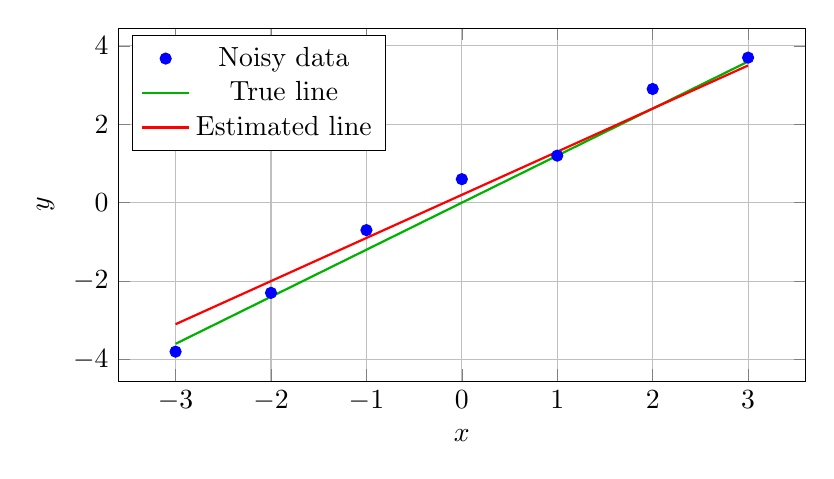
\begin{tikzpicture}
    \begin{axis}[
      width=0.85\textwidth,
      height=0.5\textwidth,
      xlabel={$x$},
      ylabel={$y$},
      legend style={at={(0.02,0.98)},anchor=north west},
      grid=major
    ]
      \addplot[only marks, mark=*, color=blue] coordinates {
        (-3,-3.8)
        (-2,-2.3)
        (-1,-0.7)
        (0,0.6)
        (1,1.2)
        (2,2.9)
        (3,3.7)
      };
      \addlegendentry{Noisy data}
      \addplot[domain=-3:3, samples=2, thick, color=green!70!black] {1.2*x};
      \addlegendentry{True line}
      \addplot[domain=-3:3, samples=2, thick, color=red] {0.2 + 1.1*x};
      \addlegendentry{Estimated line}
    \end{axis}
  \end{tikzpicture}
\end{frame}

\begin{frame}{From Simple to General Linear Regression}
  For \(n\)-dimensional inputs:
  \[
    y = \theta_0 + \theta_1 x_1 + \cdots + \theta_n x_n
  \]
  \begin{itemize}
    \item Each feature contributes linearly to the prediction.
    \item Still linear in parameters \(\theta\).
  \end{itemize}
\end{frame}

\begin{frame}{Vectorized Representation}
  Introduce dummy feature \(x_0 = 1\):
  \[
    y = \theta^T x, \quad x = [x_0, x_1, \ldots, x_n]^T
  \]
  Dimensions:
  \[
    x \in \R^{n+1}, \quad \theta \in \R^{n+1}
  \]
\end{frame}

\begin{frame}{Dataset in Matrix Form}
  Stack examples into a matrix:
  \[
    X \in \R^{m \times (n+1)}, \quad y \in \R^m
  \]
  Predictions:
  \[
    \hat{y} = X\theta
  \]
\end{frame}

\begin{frame}{Mean Squared Error (MSE)}
  \[
    \mathcal{L}(\theta) = \frac{1}{m} \sum_{i=1}^m \left(y^{(i)} - \theta^T x^{(i)}\right)^2
  \]
  \begin{itemize}
    \item Penalizes large errors more strongly.
    \item Smooth, convex, and easy to optimize.
  \end{itemize}
\end{frame}

\begin{frame}{Why Squared Loss?}
  \begin{itemize}
    \item Maximum likelihood estimator under Gaussian noise.
    \item Differentiable and convex.
    \item Leads to closed-form solutions.
  \end{itemize}
  \[
    p(y \mid x, \theta) = \mathcal{N}(\theta^T x, \sigma^2)
  \]
\end{frame}

\begin{frame}{Learning as Optimization}
  Empirical risk minimization:
  \[
    \min_{\theta} \; \mathcal{L}(\theta)
  \]
  \begin{itemize}
    \item \(\mathcal{L}(\theta)\) is a convex quadratic.
    \item Unique minimizer if \(X^T X\) is full rank.
  \end{itemize}
\end{frame}

\begin{frame}{Geometry of Least Squares}
  \begin{itemize}
    \item Column space of \(X\) defines all possible predictions.
    \item Optimal \(\hat{y}\) is orthogonal projection of \(y\) onto \(\text{col}(X)\).
    \item Residual \(r = y - X\theta^*\) satisfies \(X^T r = 0\).
  \end{itemize}
\end{frame}

\begin{frame}{Gradient of the MSE Loss}
  \[
    \nabla_\theta \mathcal{L}(\theta) = \frac{2}{m} X^T (X\theta - y)
  \]
  \begin{itemize}
    \item \(X\theta - y\): residual vector.
    \item \(X^T\): aggregates residuals by feature.
  \end{itemize}
\end{frame}

\begin{frame}{Gradient Descent}
  Iterative update:
  \[
    \theta^{(t+1)} = \theta^{(t)} - \eta \nabla_\theta \mathcal{L}(\theta^{(t)})
  \]
  \begin{itemize}
    \item Step size \(\eta\) controls progress.
    \item Converges for sufficiently small \(\eta\).
  \end{itemize}
\end{frame}

\begin{frame}{Convergence Intuition}
  \begin{itemize}
    \item Too small \(\eta\): slow progress.
    \item Too large \(\eta\): divergence or oscillation.
    \item Quadratic objectives allow theoretical convergence rates.
  \end{itemize}
\end{frame}

\begin{frame}{Gradient Descent Visualization}
  \centering
  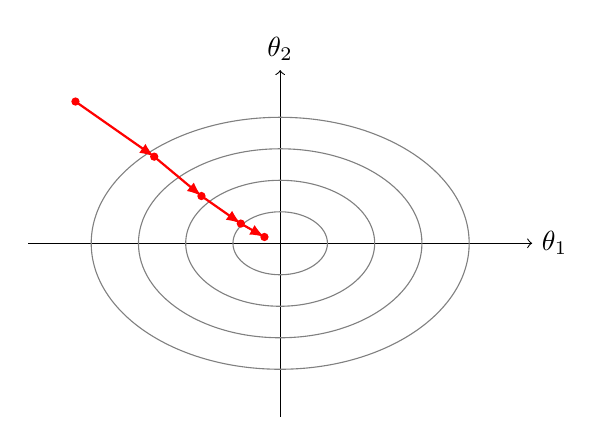
\begin{tikzpicture}
    \draw[->] (-3.2,0) -- (3.2,0) node[right] {$\theta_1$};
    \draw[->] (0,-2.2) -- (0,2.2) node[above] {$\theta_2$};

    % Contours of a quadratic loss (ellipses)
    \draw[gray] (0,0) ellipse (0.6 and 0.4);
    \draw[gray] (0,0) ellipse (1.2 and 0.8);
    \draw[gray] (0,0) ellipse (1.8 and 1.2);
    \draw[gray] (0,0) ellipse (2.4 and 1.6);

    % Optimization trajectory
    \draw[red, thick, -latex] (-2.6,1.8) -- (-1.6,1.1);
    \draw[red, thick, -latex] (-1.6,1.1) -- (-1.0,0.6);
    \draw[red, thick, -latex] (-1.0,0.6) -- (-0.5,0.25);
    \draw[red, thick, -latex] (-0.5,0.25) -- (-0.2,0.08);
    \fill[red] (-2.6,1.8) circle (1.5pt);
    \fill[red] (-1.6,1.1) circle (1.5pt);
    \fill[red] (-1.0,0.6) circle (1.5pt);
    \fill[red] (-0.5,0.25) circle (1.5pt);
    \fill[red] (-0.2,0.08) circle (1.5pt);
  \end{tikzpicture}
\end{frame}

\begin{frame}{Variants of Gradient Descent}
  \begin{itemize}
    \item \textbf{Batch GD}: uses all data per update.
    \item \textbf{Stochastic GD}: uses one example at a time.
    \item \textbf{Mini-batch GD}: uses small batches.
  \end{itemize}
  Trade-offs: computation vs.\ variance vs.\ convergence speed.
\end{frame}

\begin{frame}{When to Use Which Variant}
  \begin{itemize}
    \item Small \(m\): Batch GD is efficient and stable.
    \item Large \(m\): Mini-batch for parallelism and speed.
    \item Streaming data: Stochastic/online updates.
  \end{itemize}
\end{frame}

\begin{frame}{Closed-Form Solution: Normal Equations}
  Solve \(\nabla_\theta \mathcal{L}(\theta) = 0\):
  \[
    X^T X \theta = X^T y
  \]
  \[
    \theta^* = (X^T X)^{-1} X^T y
  \]
\end{frame}

\begin{frame}{Invertibility Conditions}
  \begin{itemize}
    \item \(X^T X\) invertible if columns of \(X\) are linearly independent.
    \item If not full rank, use pseudo-inverse:
      \[
        \theta^* = X^{\dagger} y
      \]
  \end{itemize}
\end{frame}

\begin{frame}{Normal Equations: Pros and Cons}
  \textbf{Pros}
  \begin{itemize}
    \item Exact minimizer for quadratic loss.
    \item No learning rate to tune.
  \end{itemize}
  \textbf{Cons}
  \begin{itemize}
    \item \(O(n^3)\) time for matrix inversion.
    \item Sensitive to numerical conditioning.
  \end{itemize}
\end{frame}

\begin{frame}{Optimization vs.\ Closed-Form}
  \centering
  \begin{tabular}{lcc}
    \toprule
    Method & Scalability & Flexibility \\
    \midrule
    Gradient Descent & High & High \\
    Normal Equations & Low (large \(n\)) & Medium \\
    \bottomrule
  \end{tabular}
  \vspace{0.8em}

  \begin{itemize}
    \item GD supports large-scale and regularized objectives.
    \item Closed-form is best for small, well-conditioned problems.
  \end{itemize}
\end{frame}

\begin{frame}{Feature Engineering}
  Linear in parameters does not mean linear in inputs:
  \[
    \phi(x) = [1, x, x^2, \ldots, x^d]
  \]
  \[
    y = \theta^T \phi(x)
  \]
  \begin{itemize}
    \item Enables nonlinear decision boundaries.
    \item Retains convex optimization.
  \end{itemize}
\end{frame}

\begin{frame}{Polynomial Regression Example}
  \centering
  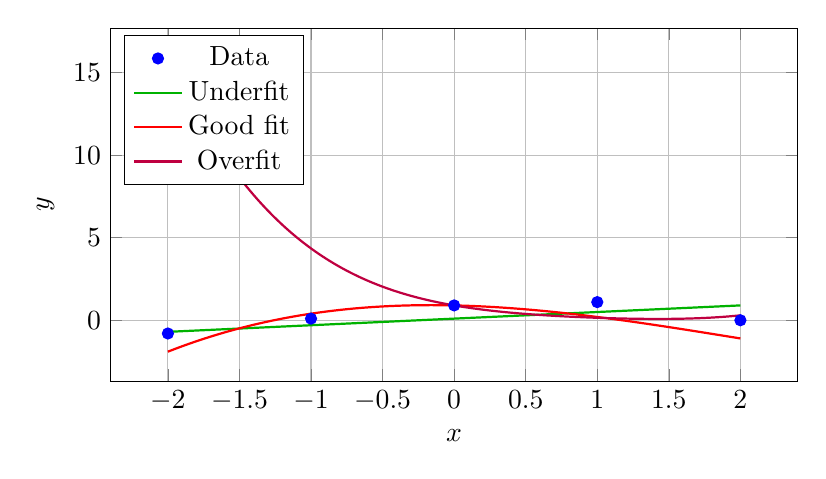
\begin{tikzpicture}
    \begin{axis}[
      width=0.85\textwidth,
      height=0.5\textwidth,
      xlabel={$x$},
      ylabel={$y$},
      legend style={at={(0.02,0.98)},anchor=north west},
      grid=major
    ]
      \addplot[only marks, mark=*, color=blue] coordinates {
        (-2,-0.8)
        (-1,0.1)
        (0,0.9)
        (1,1.1)
        (2,0.0)
      };
      \addlegendentry{Data}
      \addplot[domain=-2:2, samples=50, thick, color=green!70!black] {0.1 + 0.4*x};
      \addlegendentry{Underfit}
      \addplot[domain=-2:2, samples=200, thick, color=red] {0.9 - 0.2*x - 0.6*x^2 + 0.1*x^3};
      \addlegendentry{Good fit}
      \addplot[domain=-2:2, samples=200, thick, color=purple] {0.9 - 1.5*x + 1.2*x^2 - 0.6*x^3 + 0.15*x^4};
      \addlegendentry{Overfit}
    \end{axis}
  \end{tikzpicture}
\end{frame}

\begin{frame}{Model Complexity and Overfitting}
  \begin{itemize}
    \item Increasing degree increases flexibility and variance.
    \item Bias--variance tradeoff:
      \[
        \text{Error} = \text{Bias}^2 + \text{Variance} + \text{Noise}
      \]
    \item Overfitting: low training error, high test error.
  \end{itemize}
\end{frame}

\begin{frame}{Training vs.\ Test Error Curves}
  \centering
  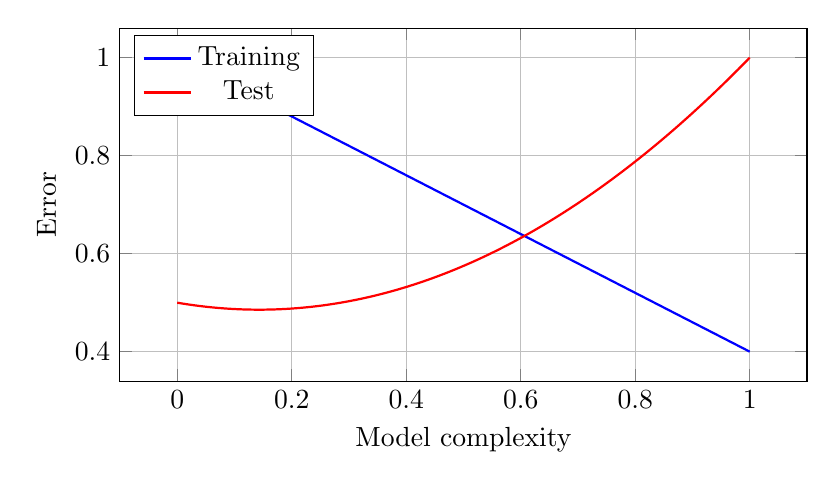
\begin{tikzpicture}
    \begin{axis}[
      width=0.85\textwidth,
      height=0.5\textwidth,
      xlabel={Model complexity},
      ylabel={Error},
      legend style={at={(0.02,0.98)},anchor=north west},
      grid=major
    ]
      \addplot[domain=0:1, samples=100, thick, color=blue] {0.9 - 0.6*x + 0.1};
      \addlegendentry{Training}
      \addplot[domain=0:1, samples=100, thick, color=red] {0.5 - 0.2*x + 0.7*x^2};
      \addlegendentry{Test}
    \end{axis}
  \end{tikzpicture}
\end{frame}

\begin{frame}{Regularization: Motivation}
  \begin{itemize}
    \item Penalize complexity to improve generalization.
    \item Encourage simpler models with smaller coefficients.
    \item Trade-off controlled by \(\lambda\).
  \end{itemize}
\end{frame}

\begin{frame}{L2 Regularization (Ridge)}
  Objective:
  \[
    \min_\theta \; \|X\theta - y\|_2^2 + \lambda \|\theta\|_2^2
  \]
  Closed form:
  \[
    \theta^* = (X^T X + \lambda I)^{-1} X^T y
  \]
  Effect: shrinks coefficients toward zero.
\end{frame}

\begin{frame}{L1 Regularization (Lasso)}
  Objective:
  \[
    \min_\theta \; \|X\theta - y\|_2^2 + \lambda \|\theta\|_1
  \]
  \begin{itemize}
    \item Encourages sparse solutions.
    \item Performs implicit feature selection.
  \end{itemize}
\end{frame}

\begin{frame}{L1 vs.\ L2: Geometry}
  \centering
  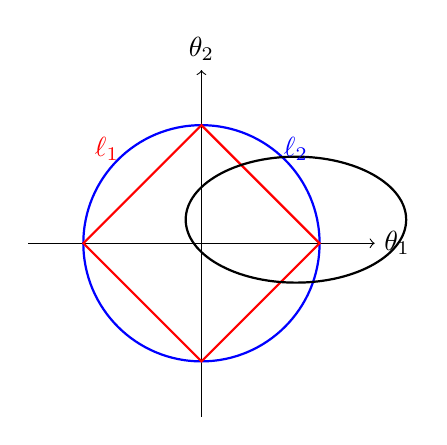
\begin{tikzpicture}[scale=1.0]
    \draw[->] (-2.2,0) -- (2.2,0) node[right] {$\theta_1$};
    \draw[->] (0,-2.2) -- (0,2.2) node[above] {$\theta_2$};
    \draw[thick, blue] (0,0) circle (1.5);
    \draw[thick, red] (0,1.5) -- (1.5,0) -- (0,-1.5) -- (-1.5,0) -- cycle;
    \draw[thick, black] (1.2,0.3) ellipse (1.4 and 0.8);
    \node[blue] at (1.2,1.2) {$\ell_2$};
    \node[red] at (-1.2,1.2) {$\ell_1$};
  \end{tikzpicture}
\end{frame}

\begin{frame}{Summary}
  \begin{itemize}
    \item Linear regression = empirical risk minimization with MSE.
    \item Optimization via gradient descent or closed-form normal equations.
    \item Feature mappings enable nonlinear trends.
    \item Regularization controls overfitting.
  \end{itemize}
\end{frame}

\begin{frame}{Looking Ahead}
  Connections to:
  \begin{itemize}
    \item Generalized linear models (logistic, Poisson).
    \item Kernel methods and RKHS regression.
    \item Linear layers inside deep networks.
  \end{itemize}
\end{frame}
